
\documentclass[aspectratio=169, 10pt]{beamer}

% Carrega preâmbulo padronizado
\input{../Preambles/header}
\usepackage{natbib}

\title[Exposição à IA no Brasil]{Exposição à Inteligência Artificial em um Mercado de Trabalho Informal}
\subtitle{Teoria e Evidências Microeconômicas para o Brasil}
\author[Marcelo Moura Freire]{Marcelo Moura Freire}
\date{2026}

\begin{document}

% -----------------------------------------------------------------------------
% Slide 1: Título
% -----------------------------------------------------------------------------
\begin{frame}[plain]
    \titlepage
\end{frame}

% -----------------------------------------------------------------------------
% Slide 2: Motivação & Contexto Brasileiro
% -----------------------------------------------------------------------------
\begin{frame}{Motivação: A Dualidade do Mercado de Trabalho Brasileiro}
    \begin{columns}[T]
        \begin{column}{0.56\textwidth}
            \textbf{O debate global sobre IA:}
            \begin{itemize}
                \item Foco em economias avançadas com alta formalidade
                e serviços corporativos \citep{eloundou2024gpts}.
                \item Premissa implícita: difusão tecnológica homogênea.
            \end{itemize}

            \vspace{0.3em}
            \textbf{A realidade estrutural do Brasil (PNAD Contínua 2026Q1):}
            \begin{itemize}
                \item \key{39,2\% de informalidade} na força ocupada.
                \item \key{35,7 milhões de pessoas (35,0\%)} em ocupações
                de baixíssima exposição à IA (quintil inferior).
                \item Forte heterogeneidade regional: formalidade varia
                de 40\% (MA/PA) a 65\% (SP/SC).
            \end{itemize}
        \end{column}

        \begin{column}{0.40\textwidth}
            \begin{block}{Questão Central}
                Como a coexistência entre \key{informalidade} e
                \key{capital humano} molda a exposição à IA em
                uma economia em desenvolvimento?
            \end{block}

            \vspace{0.4em}
            \textbf{Mecanismo Proposto:} \\
            A IA complementa o capital humano formal, mas a
            informalidade atua como barreira de absorção.
        \end{column}
    \end{columns}
\end{frame}

% -----------------------------------------------------------------------------
% Slide 3: Três Perguntas de Pesquisa
% -----------------------------------------------------------------------------
\begin{frame}{Três Perguntas de Pesquisa}
    \begin{enumerate}
        \item \textbf{Gradiente Educacional:}
        \begin{itemize}
            \item Trabalhadores mais escolarizados selecionam-se
            em postos de trabalho mais expostos à IA?
            \item O gradiente resiste ao controle de rendimento e
            covariáveis mincerianas?
        \end{itemize}
        \vspace{0.4em}
        \item \textbf{O Canal da Informalidade (Mediação):}
        \begin{itemize}
            \item A baixa exposição informal é apenas menor escolaridade,
            ou há efeito direto do \key{capital organizacional}?
        \end{itemize}
        \vspace{0.4em}
        \item \textbf{Polarização Espacial \& Heterogeneidade Regional:}
        \begin{itemize}
            \item Mercados regionais mais formais ampliam ou reduzem a
            distância de exposição entre níveis educacionais?
        \end{itemize}
    \end{enumerate}
\end{frame}

% -----------------------------------------------------------------------------
% Transição: Modelo Teórico
% -----------------------------------------------------------------------------
\transitionslide{Modelo Teórico de Alocação e Arbitragem}

% -----------------------------------------------------------------------------
% Slide 4: Estrutura do Modelo Teórico
% -----------------------------------------------------------------------------
\begin{frame}{Modelo de Designação Ocupacional (Assignment Model)}
    \begin{columns}[T]
        \begin{column}{0.50\textwidth}
            \textbf{Trabalhadores e Ocupações:}
            \begin{itemize}
                \item Escolaridade contínua: $e \in [e_{\min}, e_{\max}]$.
                \item Ocupações com exposição à IA: $\theta_j \in [0, 10]$.
                \item Regimes contratuais: $s \in \{F, I\}$ (Formal vs. Informal).
            \end{itemize}

            \vspace{0.3em}
            \textbf{Função de Produção Primitiva:}
            \begin{equation*}
                y_{js}(e) = g(e)\big(1 + \kappa_s \theta_j\big)
            \end{equation*}
            com $g'(e) > 0, g''(e) \le 0$ e $\Delta\kappa \equiv \kappa_F - \kappa_I > 0$
            ($\kappa_F \equiv \kappa_{\text{org}} > \kappa_I \equiv \kappa_{\text{ind}}$).
        \end{column}

        \begin{column}{0.46\textwidth}
            \begin{block}{Supermodularidade Estrita}
                \begin{equation*}
                    \frac{\partial^2 y}{\partial e \partial \theta} = g'(e)\,\kappa_s > 0
                \end{equation*}
                A IA complementa o capital humano do trabalhador.
            \end{block}

            \vspace{0.2em}
            \textbf{Estrutura de Custos Institucionais:}
            \begin{itemize}
                \item Formalização impõe custo fixo $c > 0$
                por trabalhador \citep{ulyssea2018firms}.
                \item $w_{jF}(e) = y_{jF}(e) - c$ e $w_{jI}(e) = y_{jI}(e)$.
            \end{itemize}
        \end{column}
    \end{columns}
\end{frame}

% -----------------------------------------------------------------------------
% Slide 5: Equilíbrio e Previsões Teóricas
% -----------------------------------------------------------------------------
\begin{frame}{Arbitragem Formal-Informal e Previsões Teóricas}
    \begin{columns}[T]
        \begin{column}{0.50\textwidth}
            \textbf{Limiar de Formalização Ocupacional:}
            \begin{equation*}
                w_{jF}(e) \ge w_{jI}(e) \iff g(e)\,\Delta\kappa\,\theta_j \ge c
            \end{equation*}
            \pause
            \begin{equation*}
                \boxed{e^*_j = g^{-1}\left(\frac{c}{\Delta\kappa\,\theta_j}\right)}
            \end{equation*}
            com $\frac{\partial e^*_j}{\partial \theta_j} < 0$.

            \begin{itemize}
                \item Maior $\theta_j$ reduz a escolaridade mínima: ganhos
                produtivos ($\Delta\kappa\,\theta_j$) amortizam o custo fixo $c$.
            \end{itemize}
        \end{column}

        \begin{column}{0.46\textwidth}
            \begin{block}{Proposição 1 (Gradiente Positivo)}
                Por supermodularidade estrita
                \citep{topkis1998supermodularity}, a alocação de
                equilíbrio $\theta^*(e)$ é crescente em $e$ ($\theta^{*\prime}(e) > 0$).
            \end{block}

            \vspace{0.3em}
            \textbf{Corolário 1 (Mediação Parcial):} \\
            A associação bruta exposição--formalidade atenua-se
            ao condicionar na escolaridade, mas retém coeficiente
            direto significativo ($\Delta\kappa > 0$).
        \end{column}
    \end{columns}
\end{frame}

% -----------------------------------------------------------------------------
% Transição: Dados e Estratégia Empírica
% -----------------------------------------------------------------------------
\transitionslide{Dados Microeconômicos e Estratégia Empírica}

% -----------------------------------------------------------------------------
% Slide 6: Microdados e Mapeamento Ocupacional
% -----------------------------------------------------------------------------
\begin{frame}{Microdados da PNAD Contínua e Construção do Escore $\theta_j$}
    \begin{columns}[T]
        \begin{column}{0.52\textwidth}
            \textbf{Base Amostral:}
            \begin{itemize}
                \item \textbf{IBGE PNAD Contínua 2026Q1}: $N = 227.629$
                indivíduos (102,1 milhões de ocupados).
                \item Pesos amostrais (\texttt{weight} / \texttt{V1028})
                em todas as estimações (WLS).
            \end{itemize}

            \vspace{0.2em}
            \textbf{Harmonização Internacional de $\theta_j$:}
            \begin{itemize}
                \item Medida O*NET-SOC (0--10) \citep{eloundou2024gpts}.
                \item $\text{O*NET} \to \text{ISCO-08} \to \text{COD (IBGE)}$.
                \item $G = 122$ grupos ocupacionais a 4 dígitos.
            \end{itemize}
        \end{column}

        \begin{column}{0.44\textwidth}
            \begin{block}{Correção de Moulton (1986)}
                Erros-padrão agrupados por \key{122 clusters}
                ocupacionais \citep{cameron2008bootstrap}.
            \end{block}

            \vspace{0.3em}
            \textbf{Controles Mincerianos:}
            \begin{itemize}
                \item Idade, idade$^2$, dummy feminina e
                vetor de raça/cor (IBGE).
            \end{itemize}
        \end{column}
    \end{columns}
\end{frame}

% -----------------------------------------------------------------------------
% Slide 7: Especificações Econométricas (2 Colunas)
% -----------------------------------------------------------------------------
\begin{frame}{Especificações Econométricas Estimadas}
    \begin{columns}[T]
        \begin{column}{0.48\textwidth}
            \textbf{Modelos no Nível Individual:}
            \vspace{0.2em}
            \begin{itemize}
                \item \textbf{S1 (Gradiente Baseline):}
                \begin{equation*}
                    \theta_{j(i)} = \alpha + \beta_1 \, e_i + \mathbf{X}_i'\boldsymbol{\gamma} + \varepsilon_i
                \end{equation*}

                \item \textbf{S2 (Controle de Rendimento):}
                \begin{equation*}
                    \theta_{j(i)} = \alpha + \beta_1 \, e_i + \beta_w \, w_i + \mathbf{X}_i'\boldsymbol{\gamma} + \varepsilon_i
                \end{equation*}
            \end{itemize}
        \end{column}

        \begin{column}{0.48\textwidth}
            \textbf{Mecanismos e Espaço:}
            \vspace{0.2em}
            \begin{itemize}
                \item \textbf{S3 (Mediação da Informalidade):}
                \begin{align*}
                    \text{informal}_i &= \alpha + \delta_1 \, \theta_{j(i)} \\
                    &+ \delta_2 \, e_i + \mathbf{X}_i'\boldsymbol{\gamma} + \varepsilon_i
                \end{align*}

                \item \textbf{S4 (Interação Regional LOO):}
                \begin{align*}
                    \theta_{j(i)} = \alpha &+ \beta_1 \, e_i + \beta_2 \big(e_i \times \text{formal}_{-i, u}^{\text{LOO}}\big) \\
                    &+ \beta_3 \, \text{formal}_{-i, u}^{\text{LOO}} + \mathbf{X}_i'\boldsymbol{\gamma} + \varepsilon_i
                \end{align*}
            \end{itemize}
        \end{column}
    \end{columns}
\end{frame}

% -----------------------------------------------------------------------------
% Transição: Resultados Empíricos
% -----------------------------------------------------------------------------
\transitionslide{Resultados Empíricos e Mecanismos}

% -----------------------------------------------------------------------------
% Slide 8: Resultado 1 — Gradiente Educacional
% -----------------------------------------------------------------------------
\begin{frame}{Resultado 1: Gradiente Escolaridade--Exposição ($\hat{\beta}_1 = 0{,}23$)}
    \begin{columns}[T]
        \begin{column}{0.50\textwidth}
            \textbf{Estimação Individual ($N = 227.629$):}
            \begin{itemize}
                \item \textbf{S1 Baseline:} $\hat{\beta}_1 = \mathbf{0{,}23}$
                (EP $0{,}03; p < 0{,}001; R^2 = 0{,}25$).
                \item 4 anos de estudo elevam exposição em $\sim 1$ ponto.
                \item \textbf{S2 Salário:} $\hat{\beta}_1 = \mathbf{0{,}21}$ (EP $0{,}03$);
                Rendimento: $\hat{\beta}_w = \mathbf{0{,}043}$ ($p < 0{,}001$).
            \end{itemize}

            \vspace{0.1em}
            \begin{block}{Limites de Oster (2019)}
                $\delta = \mathbf{1{,}64} > 1$ sob $R_{\max} = 1{,}3 R^2$:
                seleção em não observáveis precisaria ser 64\%
                superior aos controles para anular $\hat{\beta}_1$.
            \end{block}
        \end{column}

        \begin{column}{0.46\textwidth}
            \centering
            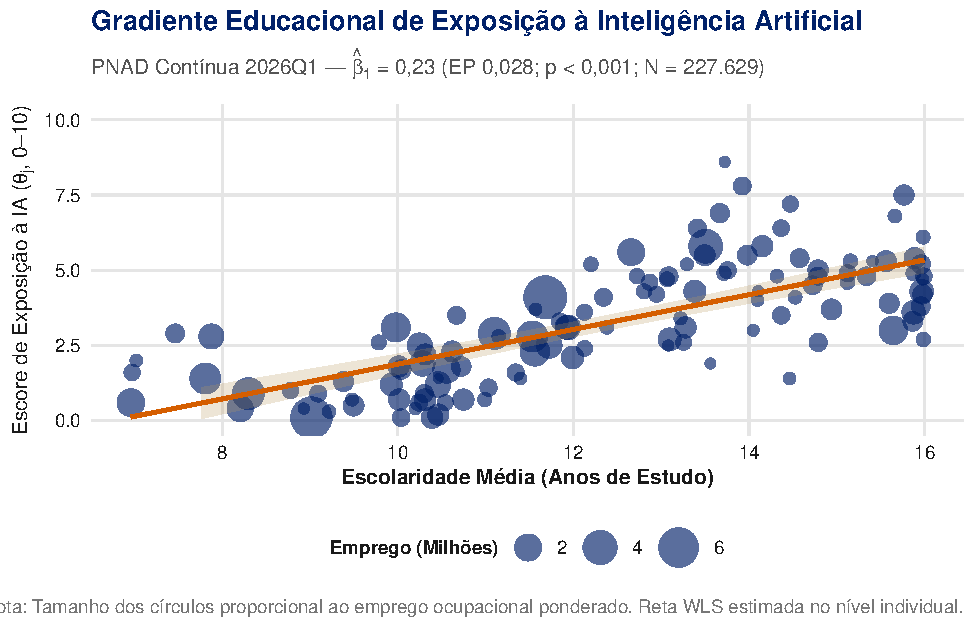
\includegraphics[width=\linewidth]{../Figures/fig1_gradiente}
        \end{column}
    \end{columns}
\end{frame}

% -----------------------------------------------------------------------------
% Slide 9: Resultado 2 — Mediação e Capital Organizacional
% -----------------------------------------------------------------------------
\begin{frame}{Resultado 2: Mediação Parcial da Informalidade (Corolário 1)}
    \begin{columns}[T]
        \begin{column}{0.50\textwidth}
            \textbf{Decomposição Linear Exata:}
            \begin{itemize}
                \item \textbf{S3a (Bruta):} $\hat{\delta}_1 = \mathbf{-6{,}23}$ p.p.
                por ponto de $\theta_j$ (EP $0{,}99; p < 0{,}001$).
                \item \textbf{S3 (Cond.):} $\hat{\delta}_1 = \mathbf{-3{,}91}$ p.p.
                (EP $0{,}96$) e $\hat{\delta}_2 = \mathbf{-2{,}61}$ p.p./ano.
            \end{itemize}

            \pause
            \vspace{0.2em}
            \begin{block}{Decomposição de Canais: $\frac{-3{,}91}{-6{,}23} = \mathbf{62{,}8\%}$}
                \begin{itemize}
                    \item \key{37,2\% Atenuação}: Seleção em tarefas cognitivas.
                    \item \key{62,8\% Efeito Direto}: Governança,
                    escala de dados e capital organizacional ($\Delta\kappa > 0$).
                \end{itemize}
            \end{block}
        \end{column}

        \begin{column}{0.46\textwidth}
            \centering
            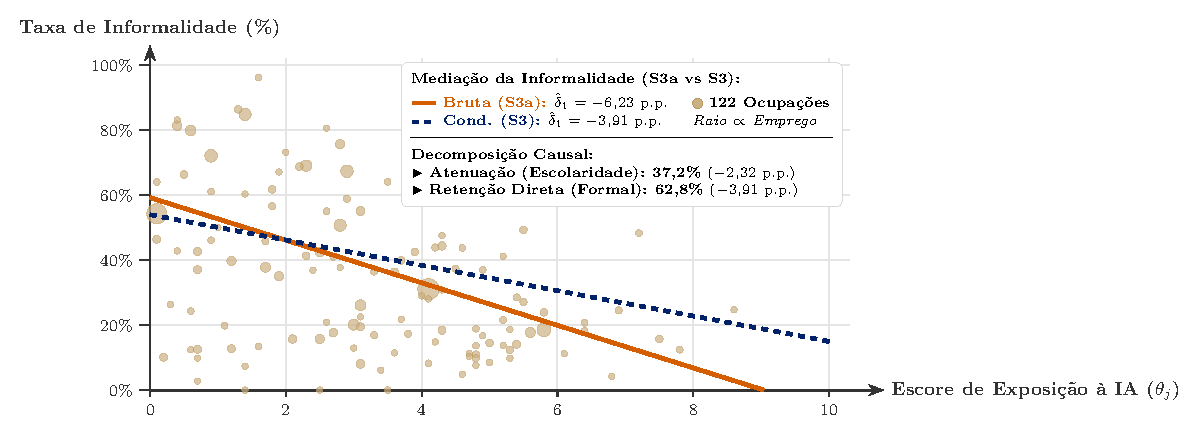
\includegraphics[width=\linewidth]{../Figures/fig2_mediacao}
        \end{column}
    \end{columns}
\end{frame}

% -----------------------------------------------------------------------------
% Slide 10: Resultado 3 — Polarização Geográfica
% -----------------------------------------------------------------------------
\begin{frame}{Resultado 3: Polarização Espacial e Formalidade Regional (S4)}
    \begin{columns}[T]
        \begin{column}{0.50\textwidth}
            \textbf{Estimativas da Interação Regional (S4):}
            \begin{itemize}
                \item Interação $\text{Esc} \times \text{Formal}$:
                $\hat{\beta}_2 = \mathbf{+0{,}28}$ (EP $0{,}06; p < 0{,}001$).
                \item Efeito Principal Formalidade:
                $\hat{\beta}_3 = \mathbf{-3{,}10}$ (EP $0{,}77; p < 0{,}001$).
            \end{itemize}

            \vspace{0.2em}
            \textbf{Derivada Total:} $\frac{\partial \theta}{\partial \text{formal}_u} = -3{,}10 + 0{,}28 \, e_i$

            \pause
            \vspace{0.1em}
            \begin{block}{Limiar Crítico de Polarização: $e^* = 11{,}14$ anos}
                \begin{itemize}
                    \item $e_i = 8$ anos (Fund.):
                    $\frac{\partial \theta}{\partial \text{formal}_u} = \mathbf{-0{,}86}$ pt. (segregação manual).
                    \item $e_i = 16$ anos (Sup.):
                    $\frac{\partial \theta}{\partial \text{formal}_u} = \mathbf{+1{,}38}$ pt. (complementaridade).
                \end{itemize}
            \end{block}
        \end{column}

        \begin{column}{0.46\textwidth}
            \centering
            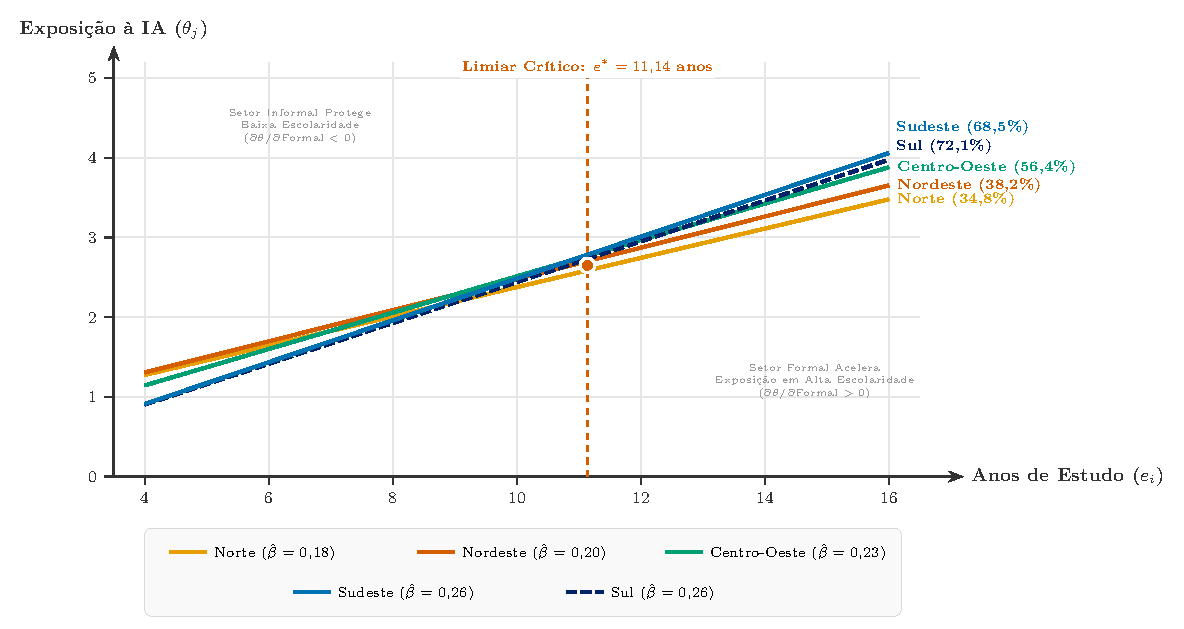
\includegraphics[width=\linewidth]{../Figures/fig3_regional_slopes}
        \end{column}
    \end{columns}
\end{frame}

% -----------------------------------------------------------------------------
% Slide 11: Robustez e Sensibilidade
% -----------------------------------------------------------------------------
\begin{frame}{Bateria de Robustez Econométrica (R1--R7)}
    \begin{columns}[T]
        \begin{column}{0.50\textwidth}
            \textbf{Sensibilidade e Especificação:}
            \begin{itemize}
                \item \textbf{Amostra e Outliers:} Winsorização 1\%/99\% ($\hat{\beta}_1 = 0{,}23$); Exclusão p99 ($\hat{\beta}_1 = 0{,}22$); Exclusão dos 9 grupos COD ($\hat{\beta}_1 \in [0{,}19; 0{,}26]$).
                \item \textbf{Forma Funcional (R4):} $\log(1+\theta)$ ($\hat{\beta}_1 = 0{,}07; p < 0{,}001$).
                \item \textbf{Pesos Amostrais (R1):} OLS não-ponderado ($\hat{\beta}_1 = 0{,}21$).
            \end{itemize}

            \vspace{0.2em}
            \begin{block}{Wild Cluster Bootstrap (27 UFs)}
                $p < 0{,}001$ com 1.000 replicações para a interação regional.
            \end{block}
        \end{column}

        \begin{column}{0.46\textwidth}
            \centering
            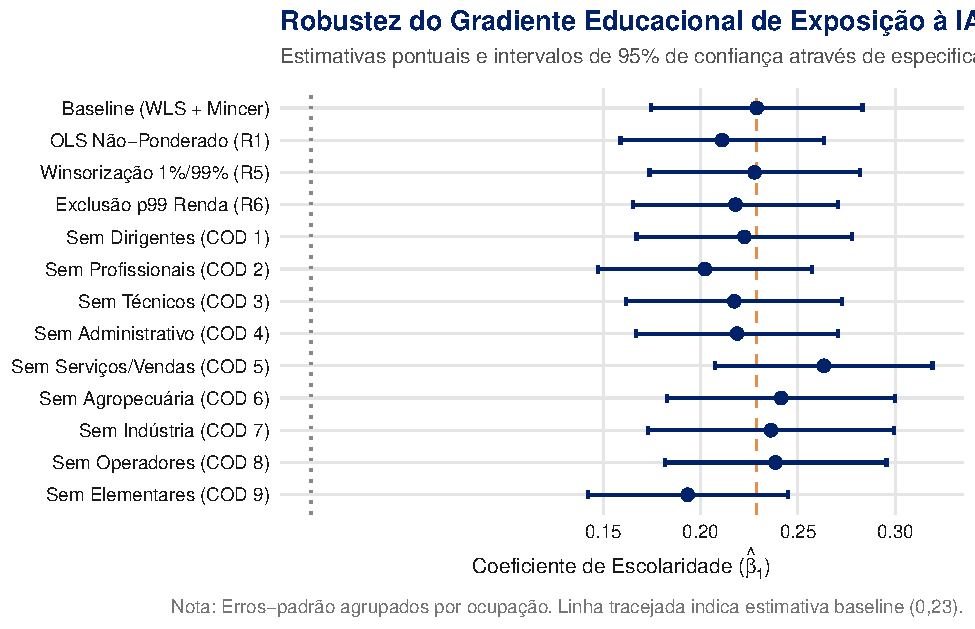
\includegraphics[width=\linewidth]{../Figures/fig5_robustez_forest}
        \end{column}
    \end{columns}
\end{frame}

% -----------------------------------------------------------------------------
% Slide 12: Conclusões e Implicações de Política
% -----------------------------------------------------------------------------
\begin{frame}{Conclusões e Implicações de Política Pública}
    \begin{columns}[T]
        \begin{column}{0.48\textwidth}
            \textbf{Principais Achados:}
            \begin{enumerate}
                \item \textbf{Gradiente Positivo:} A IA complementa postos de
                alta qualificação no Brasil ($\hat{\beta}_1 = 0{,}23$).
                \item \textbf{Canal Organizacional:} Informalidade como barreira
                de absorção (62,8\% retido).
                \item \textbf{Polarização Geográfica:} Formalização regional
                amplia o hiato ($e^* \approx 11$ anos).
            \end{enumerate}
        \end{column}

        \begin{column}{0.48\textwidth}
            \begin{block}{Recomendações de Política}
                \begin{itemize}
                    \item \textbf{Qualificação Digital na Base:} Evitar a
                    exclusão permanente dos 35,7 milhões de informais.
                    \item \textbf{Incentivos à Transição Formal:} Políticas
                    com foco em infraestrutura corporativa (PMEs).
                \end{itemize}
            \end{block}
        \end{column}
    \end{columns}
\end{frame}

% -----------------------------------------------------------------------------
% Slide 13: Referências
% -----------------------------------------------------------------------------
\begin{frame}{Referências Selecionadas}
    \footnotesize
    \bibliographystyle{plainnat}
    \bibliography{../paper/references}
\end{frame}

\end{document}
